\documentclass[letterpaper,onside,11pt]{book}

%	Paquetes
\usepackage[paperwidth=17cm, 
			paperheight=22.5cm, 
			bottom=2.5cm, 
			right=2.5cm]{geometry}
\usepackage[utf8]{inputenc}
\usepackage[spanish]{babel}
%\usepackage{algorithm}
\usepackage{amsmath}
\usepackage{amssymb}
\usepackage{amsthm}
\usepackage{hyperref}
\usepackage{graphicx}
\usepackage{subfig}
\usepackage[toc,page]{appendix}
\usepackage{booktabs}
%\usepackage{algorithm2e}
 
%	Estilo de bibliografia
\usepackage[round]{natbib}
%\bibliographystyle{apalike}
\bibliographystyle{chicago}
%\bibliographystyle{unsrtnat}
 
% para su uso en maketitle
\title{T\'itulo}
\author{Autor}
\date{\today}
 
%	Commands
\renewcommand{\chaptername}{Cap\'itulo}
%\renewcommand{\figurename}{Gr\'afica}
\renewcommand\spanishfigurename{Gr\'afica} 
\usepackage{setspace}
%\singlespacing        %% 1-spacing (default)
\onehalfspacing       %% 1,5-spacing
%\doublespacing        %% 2-spacing
\pagestyle{plain}

%
%	Documento
%
\begin{document}
 
%	No MAKETITLE
%\maketitle	% comenta esta instruccion para la version final

\begin{titlepage}
	\begin{center}
		
		\textsc{\Large Instituto Tecnol\'ogico Aut\'onomo de M\'exico}\\[4em]
		
		%Figura
		\begin{center}
			
\includegraphics{DocumentosLaTex/ITAM_2016.png}
		\end{center}
		
		\vspace{2em}
		
		{\sc \huge {\bf T\'itulo}}\\[4em]
		
		\textsc{\large Tesis}\\[1em]
		
		\textsc{que para obtener el t\'itulo}\\[1em]
		
		\textsc{Licenciado en <<carrera>>}\\[1em]
		
		\textsc{presenta}\\[1em]
		
		\textsc{\Large Autor}\\[1em]
		
		\textsc{\large Asesor: ...}
		
	\end{center}
	
	\vspace*{\fill}
	\textsc{Ciudad de M\'exico \hspace*{\fill} 2017}
	
\end{titlepage}

%	
\tableofcontents

%	Capitulos
\chapter{Introducci\'on}
 

\section{Antecedentes}

\section{Proceso de aprendizaje}  


\subsection{El proceso de aprendizaje en la inferencia estadística}

 Algunas expresiones \cite{AbramowitzStegun_Handbook}
 
 o 
 
 \citep{Amado}
 
 o
 
 \citeauthor{Bandorff_Nielsen}
 
 o 
 
 \cite{Pandey_Pulastya, Ross_Book}
 
 
\begin{eqnarray}
	f(y*|\overline{y})&=&\int_{S_{\theta}}f(y* \wedge \theta |\overline{y})d\theta\nonumber\\
	&=&\int_{S_{\theta}}f(y* | \theta \wedge \overline{y})\Pi(\theta) d\theta,
\end{eqnarray}  
donde $y*$ bla bla bla $Y$, y $\theta$ bla bla bla.

Algunas im\'agenes...

\begin{figure}
	\caption{Descripci\'on...}
	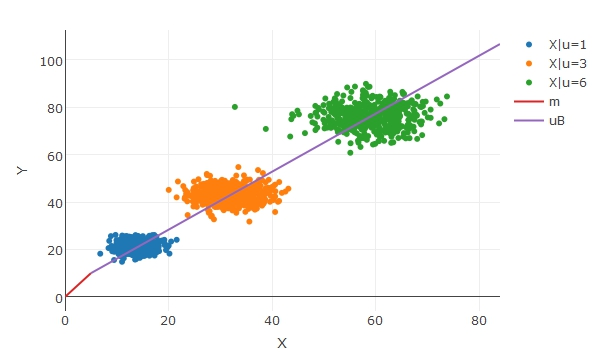
\includegraphics[scale=0.75]{Figuras/bm}
\end{figure}


Una tabla



\begin{table}[h!]
	\centering
	\caption{Descripci\'on.}
	\label{tab:table1}
	\begin{tabular}{l|c||r}
		1 & 2 & 3\\
		\hline
		a & b & c\\
	\end{tabular}
\end{table}


\begin{table}[h!]
	\centering
	\caption{Descripci\'on...}
	\label{tab:table1}
	\begin{tabular}{ccc}
		\toprule
		Some & actual & content\\
		\midrule
		prettifies & the & content\\
		as & well & as\\
		using & the & booktabs package\\
		\bottomrule
	\end{tabular}
\end{table}


Y algoritmos

%\begin{algorithm}[H]
%	\SetAlgoLined
%	\KwResult{Write here the result }
%	initialization\;
%	\While{While condition}{
%		instructions\;
%		\eIf{condition}{
%			instructions1\;
%			instructions2\;
%		}{
%		instructions3\;
%	}
%}
%\caption{How to write algorithms}
%\end{algorithm}




%	Bibliografia
\medskip
\addcontentsline{toc}{chapter}{Bibliograf\'ia}
\bibliography{tesis_itam_bibliografia}


%	Apendices
\appendix
%\input{Apendice1}

\end{document}
